\documentclass{article}
\usepackage[main,final]{neurips_2026}
\makeatletter
\renewcommand{\@noticestring}{}
\makeatother
\usepackage[utf8]{inputenc}
\usepackage[T1]{fontenc}
\usepackage{hyperref}
\usepackage{url}
\usepackage{booktabs}
\usepackage{amsmath}
\usepackage{amsfonts}
\usepackage{graphicx}
\usepackage{microtype}
\usepackage{xcolor}
\usepackage{multirow}
\usepackage{float}

\title{A Controlled Study of LLM Post-Training:\\
DPO, PPO, GRPO, Safety, and Reward Sources}
\author{Daniyal Hussain Shah}

\begin{document}
\maketitle

\begin{abstract}
This study compares direct preference optimization (DPO), proximal policy optimization (PPO), group relative policy optimization (GRPO), safety behavior, and two reward sources for mathematical reasoning, all under one constrained experimental setup. The main result is negative but still useful: the implementations gave the expected optimization signals, but most final policies stayed close to their starting checkpoints and did not show a reliable gain in quality. DPO reached 63.1\% reference-adjusted preference accuracy, but a length-controlled evaluation showed that its strongest behavior was a direction-specific preference for shorter answers. PPO clipping was activated in a fixed-batch stress test but not during ordinary updates. GRPO removed the critic, however its length normalization changed which completions dominated the gradient. On XSTest, all policies refused harmful prompts often, but a manual audit found a 36.7\% over-refusal rate on safe prompts which the automatic judge missed completely. On mathematics, neither verifiable rewards nor AI feedback improved GSM8K accuracy, and controlled perturbations showed that the AI judge mostly ignored answer correctness. These results show why training loss, reward and judge agreement need to be kept seperate from task performance. Code, configurations, logs, and machine-readable results are available at \url{https://github.com/syeddaniyalg/atml-pa2}.
\end{abstract}

\section{Introduction}
Post-training methods are different in what feedback they use and how directly that feedback reaches the policy. DPO learns from fixed preference pairs without any online generation \citep{rafailov2023dpo}. PPO generates responses, estimates returns with a critic, and clips the policy updates \citep{schulman2017ppo,ouyang2022training}. GRPO replaces the critic with rewards that are normalized inside a sampled group \citep{shao2024deepseekmath}. Reinforcement learning with verifiable rewards (RLVR) uses an exact task signal, while reinforcement learning from AI feedback (RLAIF) uses a learned judge \citep{bai2022constitutional,lee2024rlaif}.

The experiments try to answer five concrete questions. First, does DPO learn real preference quality or just a shortcut based on answer length? Second, when the online budget is small do PPO clipping and KL control actually constrain the policy? Third, what changes when GRPO removes the critic, changes the group size, or changes the length normalization? Fourth, do the resulting policies refuse harmful requests without also refusing harmless ones? Fifth, is exact mathematical verification a more useful learning signal than an AI preference judge?

The analysis separates three quantities that are easy to mix up: an optimizer diagnostic, a feedback score, and the final task performance. A clipping operator that works does not mean clipping affected the training. A higher reward does not mean improvement if there is no baseline from before training. High judge agreement can also be meaningless if most of the comparisons are ties. This distinction matters here because the update budgets are deliberately small, so many of the policy changes are also weak.

\section{Experimental protocol}
\paragraph{Shared stack.}
All policies start from Qwen2.5-1.5B-Instruct. The trainable policy parameters are LoRA adapters on the query and value projections, with rank 8, scaling parameter $\alpha=16$, and dropout 0.05. The reward model is \texttt{qwen2.5-1.5b-rm-ultrafeedback} and the pairwise judge is Qwen2.5-3B-Instruct. PPO uses Qwen2.5-0.5B-Instruct with the same LoRA dimensions plus a scalar value head. Models are frozen and loaded in 4-bit form when it is supported. Unless a task says otherwise, generation uses temperature 0.7, top-$p$ 0.9, seed 6304, and fixed prompt IDs. The training and evaluation artifacts record samples, checkpoints, aggregate tables and plots.

\paragraph{DPO.}
The standard preference split has 1,500 training and 300 evaluation pairs, and 1,446 and 290 of them pass preprocessing. A second 1,500-pair training set has 500 intended examples in each length relation: similar length, preferred answer longer, and rejected answer longer. Only 37 examples are shared between the two training sets, so this comparison changes both the length distribution and most of the pair identities. The controlled evaluation has 237 usable pairs, which are 80 similar-length, 78 preferred-longer, and 79 rejected-longer. DPO runs for one epoch with batch size 2, gradient accumulation 8, learning rate $2\times10^{-5}$, and $\beta=0.1$. A 600-example fork varies $\beta\in\{0.03,0.1,0.3\}$.

\paragraph{PPO and GRPO.}
Both methods use a 1,200-prompt training pool and a 200-prompt held-out set. The standard run does 20 updates on 20 distinct prompts. PPO samples one response per prompt and takes two PPO epochs, so it trains on 20 trajectories and not eight responses per prompt. PPO uses policy learning rate $3\times10^{-6}$, clipping $\epsilon=0.2$, KL coefficient 0.1, $\gamma=1$, and GAE $\lambda=0.95$. The value adapter and head use learning rates $10^{-4}$ and $3\times10^{-4}$. GRPO samples $K=4$ responses per prompt, which gives 80 trajectories, and uses one update epoch, learning rate $5\times10^{-6}$, $\epsilon=0.2$, and KL coefficient 0.1. The forks test PPO clipping $\epsilon\in\{0.05,0.2,0.5\}$, KL coefficients $\{0,0.1,0.2\}$, GRPO group sizes $K\in\{2,4,8\}$, and canonical versus fixed-denominator normalization.

\paragraph{Safety and mathematics.}
Safety evaluation uses all 450 XSTest prompts, which are 250 safe prompts in ten categories and 200 unsafe prompts in eight categories \citep{rottger2023xstest}. Each of the four fixed policies, SFT, DPO, PPO, and GRPO, is decoded greedily and labeled by the 3B judge. A blind manual audit covers 60 responses, balanced between safe and unsafe prompts. Mathematical evaluation uses 300 GSM8K examples and 100 SVAMP examples. RLVR gets an exact reward only when the final output matches the required \texttt{\#\#\#\# number} form and value. RLAIF uses six pairwise judge calls for each four-response group and does not get the gold answer. A 100-example diagnostic set applies four controlled changes to 20 base problems: corrupted reasoning, a wrong final answer, persuasive filler, and a gold-number distractor followed by a wrong final answer.

\paragraph{Metrics.}
DPO preference accuracy is the fraction of pairs that have a positive reference-adjusted margin
\begin{equation}
m=[\log\pi(y^+|x)-\log\pi_{\mathrm{ref}}(y^+|x)]-[\log\pi(y^-|x)-\log\pi_{\mathrm{ref}}(y^-|x)].
\end{equation}
It measures if training moves the policy toward the preferred answer relative to the frozen reference, and not whether the raw base model already preferred that answer. PPO and GRPO report reward-model score, sampled KL, entropy, length, clipping, and critic quality where it is relevant. Mathematics reports exact answer accuracy, output-format rate, and pairwise judge outcomes. Safety reports the safe-answer rate on safe prompts and the justified-refusal rate on unsafe prompts.

\section{Task 1: Direct preference optimization}
The standard DPO policy reaches 63.1\% reference-adjusted preference accuracy on 290 held-out pairs, with loss 0.674 and sampled KL 0.054 per sequence. The generated response length is 170 tokens and only 4 of 10 word-limit prompts follow the limit. The short $\beta$ forks reach 62.1\%, 63.4\%, and 62.4\% for $\beta=0.03$, 0.1, and 0.3. Their generated lengths stay between 169.7 and 170.0 tokens. So the sweep does not show a monotonic strength effect. The slightly negative sampled KL estimates are finite-sample estimates close to zero, they are not evidence of a meaningful negative divergence.

\begin{figure}[H]
  \centering
  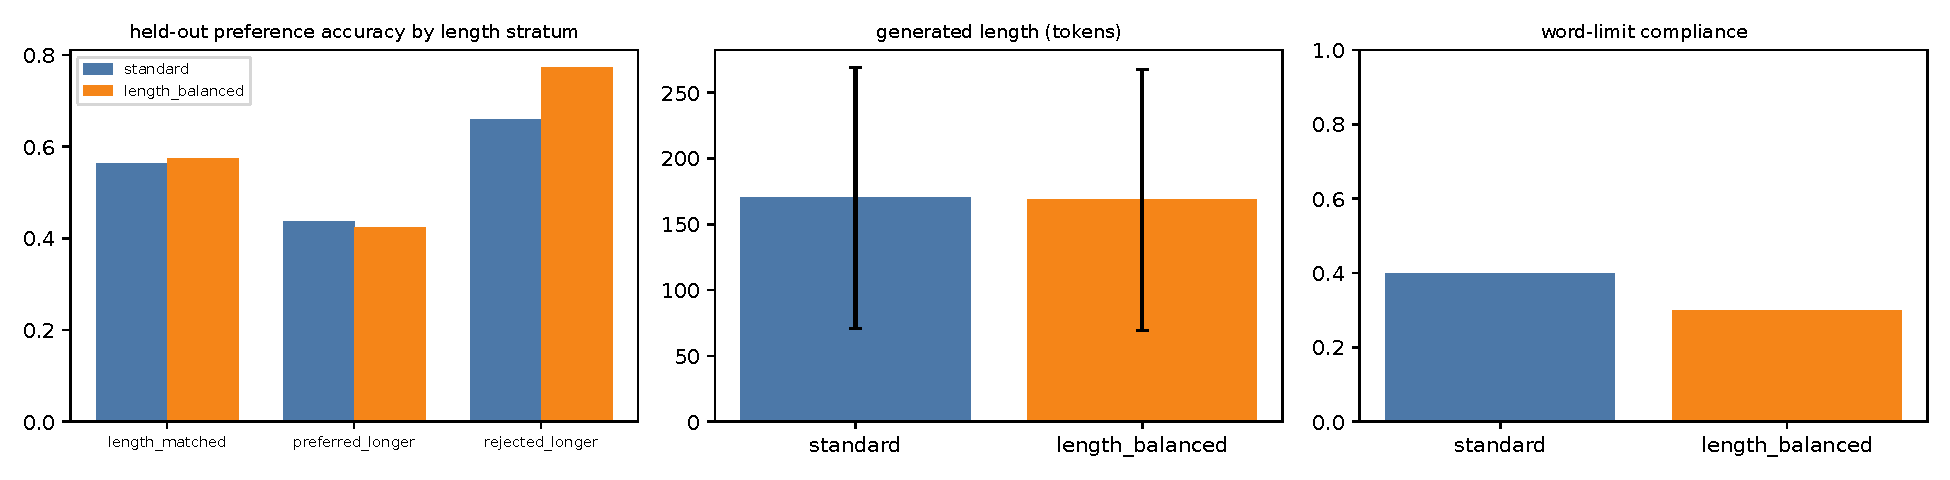
\includegraphics[width=\linewidth]{figures/task1_length_confounding.pdf}
  \caption{Length-controlled DPO evaluation. Balancing does not improve the preferred-longer cases. Its entire net gain is in the rejected-longer group, while the average generated length stays unchanged and word-limit compliance falls.}
  \label{fig:dpo-length}
\end{figure}

Table~\ref{tab:dpo-length} shows the main result of Task 1. On similar-length pairs, the two policies differ by only one correct decision. When the preferred answer is longer, the balanced model loses one decision. When the rejected answer is longer, it gains nine decisions, from 52/79 to 61/79. So all nine additional correct predictions come from cases where choosing the shorter answer is the correct one. This is not a general quality improvement and it is not evidence that the model learned to reason about length. It is just a stronger movement in the shorter-answer direction.

\begin{table}[H]
\caption{DPO accuracy by answer-length relation. The counts make it clear that the 65.8\% to 77.2\% jump is nine examples, all in one direction.}
\label{tab:dpo-length}
\centering
\small
\begin{tabular}{lrrrr}
\toprule
Relation & $n$ & Standard & Balanced & Correct-count change \\
\midrule
Similar length & 80 & 56.2\% & 57.5\% & $45\rightarrow46$ \\
Preferred answer longer & 78 & 43.6\% & 42.3\% & $34\rightarrow33$ \\
Rejected answer longer & 79 & 65.8\% & 77.2\% & $52\rightarrow61$ \\
\bottomrule
\end{tabular}
\end{table}

Two checks help us avoid overclaiming. First, both policies generate almost the same mean length, about 170 versus 169 tokens. The balanced policy is also worse on explicit word limits, 30\% versus 40\%. So the pairwise shift does not turn into generally shorter or better controlled generations. Second, the balanced training set is not a reweighting of the same pairs. With only 37 shared examples, the pair content and the length balance change together. The result supports a directional length effect, but it can not identify length balancing as the only cause.

There is also no raw pre-training accuracy for the reference model. Before training, the reference-adjusted margin is exactly zero by definition, so the reported metric only measures the direction of the update. A raw summed-log-probability and length-normalized evaluation of the base, standard, and balanced policies would be the right follow-up. This missing baseline does not invalidate the observed nine-example shift but it stops us from claiming that DPO improved over the original model.

A concrete example shows the instruction-following side of this. For the prompt ``Explain the role of a learning rate in at most 35 words,'' the standard DPO policy answers ``A learning rate is a crucial hyperparameter in machine learning and deep learning algorithms that determines the step size at each iteration\ldots'' and keeps going to 82 words, more than twice the limit. The balanced policy gives the same 82-word answer. Both policies also write 50 words for ``Explain gradient descent in under 35 words.'' The pairwise shift in Table~\ref{tab:dpo-length} did nothing to fix these length-limit failures.

\section{Task 2: Proximal policy optimization}
PPO completes its online loop, but the experiment does not show a performance gain. The held-out reward is 1.427 on 200 prompts, the mean response length is 303 tokens, truncation is 10\%, and sampled KL is 0.0055 per sequence. There is no raw-policy held-out reward measured with the same pipeline, so 1.427 is a final score and not an estimate of improvement. Open-ended prompts also do not have a natural accuracy metric.

The critic is the clearest limitation. On a 32-sample midpoint check, explained variance is $-3.672$ and return-value correlation is $-0.061$. A useful critic should at least follow which sampled returns are larger, and this critic does not. Its noisy advantages can weaken or even reverse the policy signal. The cause is concrete: the run only sees 20 trajectories and asks both the critic and the policy to learn from them. Sharing trajectories is normal practice in PPO, so the problem is the very small and diverse sample, not the fact that both models use it.

\begin{figure}[H]
  \centering
  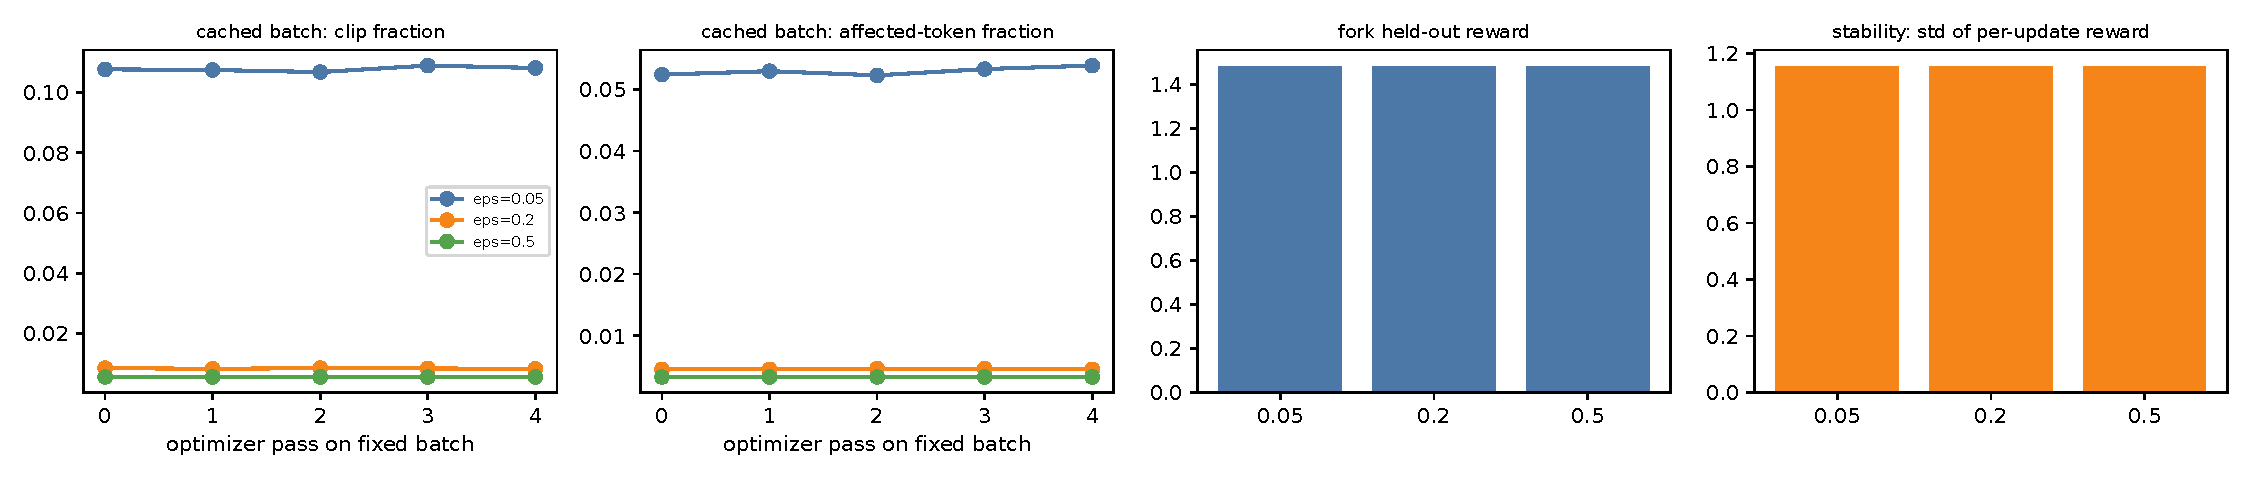
\includegraphics[width=\linewidth]{figures/task2_clipping_study.pdf}
  \caption{PPO clipping study. A repeated fixed-batch probe activates the clipping rule, especially at $\epsilon=0.05$, but the ordinary eight-update forks have zero training clip fraction and identical held-out rewards.}
  \label{fig:ppo-clip}
\end{figure}

Clipping behaves correctly when a batch is reused on purpose. Across four fixed-batch optimizer passes, $\epsilon=0.05$ clips 10.8\% of tokens and affects 5.2\% of sequences, and the corresponding numbers are 0.9\% and 0.5\% for $\epsilon=0.2$, and 0.6\% and 0.3\% for $\epsilon=0.5$. During the normal forks however the clip fraction is zero and all three settings end at reward 1.482. The update ratios never reach the clipping boundary, so changing the boundary can not change the training.

The KL forks are weak in a similar way: coefficients 0, 0.1, and 0.2 give held-out rewards 1.434, 1.482, and 1.410, with no monotonic relation. Their sampled sequence KL values stay close to zero. These differences should not be used to rank the methods, because each setting has one short run, the policy movement is tiny, and the held-out reward varies by about 1.5 accross examples. The safe conclusion is that the PPO mechanics are there, but the budget is too small for clipping, KL control, or the critic to shape a clear outcome.

A held-out example shows how reward and instruction following can come apart. For the prompt ``could you write in just 50 words the best way of PR messaging to reach top Journalists in Europe?'' the PPO policy answers ``To effectively reach top European journalists for press releases: 1. **Know Your Audience**: Tailor content that resonates with their interests and expertise\ldots'' and continues as a numbered list to 132 words. The reward model still gives it 3.95, the third highest of the 200 held-out prompts.

\section{Task 3: Group relative policy optimization}
GRPO removes the learned critic and gets advantages by comparing responses to the same prompt. The standard run generates four responses for each of 20 prompts, which is 80 trajectories and 15,264 response tokens. Its held-out reward is 1.272, the mean length is 260, truncation is 21.5\%, and sampled KL is 0.0347 per sequence. Like PPO, there is no raw-policy held-out baseline, so this is not evidence of an increase. The second half of training has a higher mean reward than the first, 1.375 versus 0.276, but each update uses a different prompt. Prompt difficulty and learning are mixed together, so this trend is not a learning curve.

Larger groups increase the reward spread inside a group but barely reduce the useless groups. With equal generation budget, the informative-group rates are 95.0\%, 95.8\%, and 95.8\% for $K=2,4,8$, while the reward standard deviation rises from 0.392 to 0.551 and 0.619. Hard prompts stay near 87.5\% informative at every size. Once $K=4$ almost always has a reward contrast, doubling the group mostly spends computation on extra samples instead of creating more updates.

\begin{figure}[H]
  \centering
  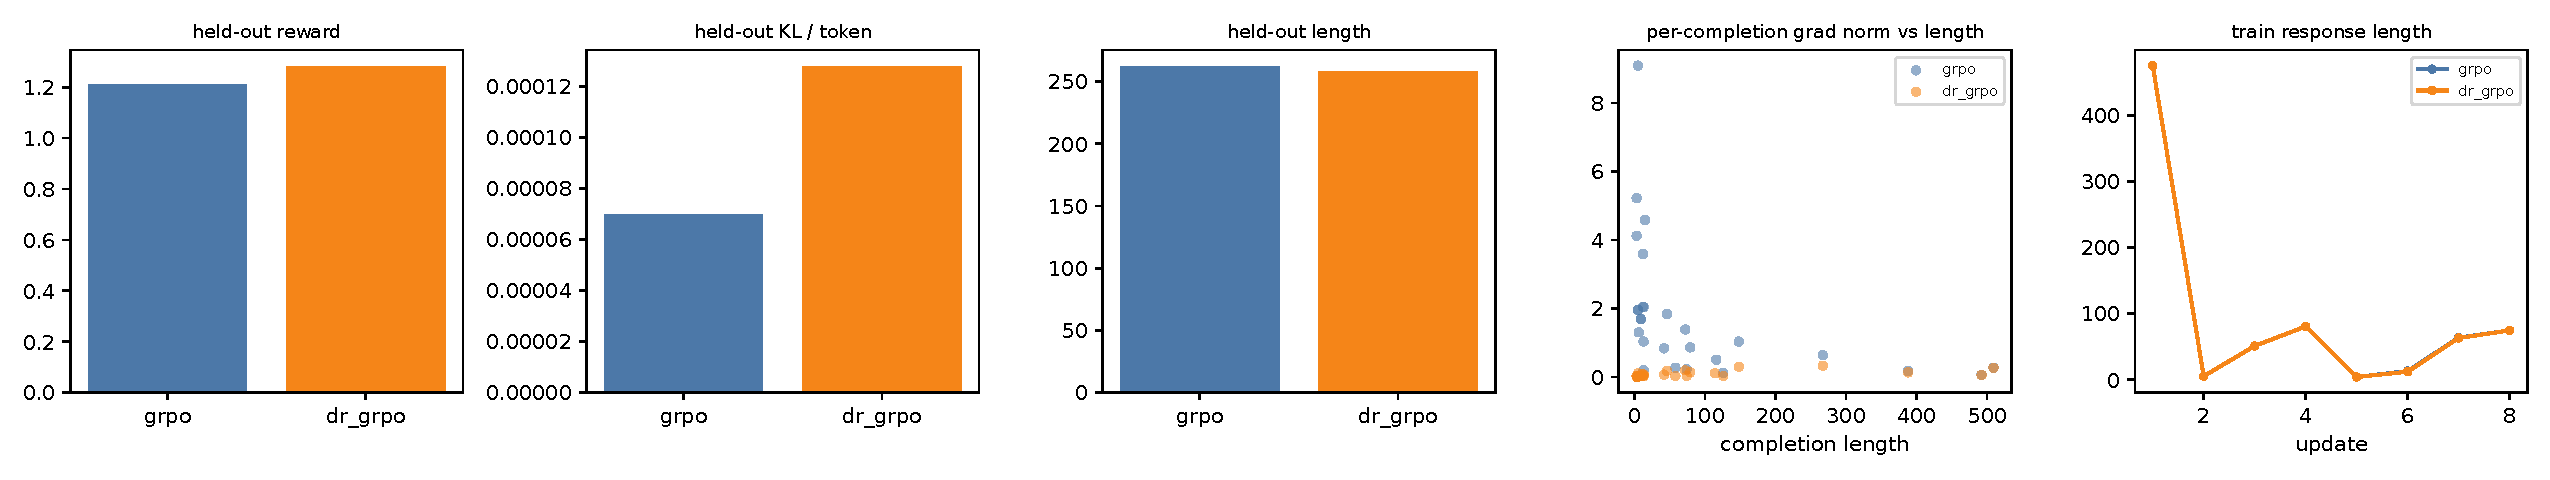
\includegraphics[width=\linewidth]{figures/task3_normalization.pdf}
  \caption{GRPO normalization ablation. The small reward difference is not reliable, but the gradient allocation reverses. Canonical normalization emphasizes short completions, while the fixed 512-token denominator lets long completions accumulate more gradient.}
  \label{fig:grpo-norm}
\end{figure}

Normalization changes the optimization bias more clearly than it changes the held-out reward. Canonical GRPO divides each completion contribution by its own token count. Its short-completion gradient norm is 2.116 versus 0.915 for long completions, a ratio of 2.31, and the length-gradient Spearman correlation is $-0.260$. The fixed-denominator variant divides by 512. Its short and long gradient norms are 0.033 and 0.144, a ratio of 0.23, with correlation $+0.743$. Canonical normalization gives each completion a similar total weight, which makes every token in a short answer count more. A fixed denominator gives each token the same scale, so long answers collect more total weight. This explains the reversal directly.

Held-out reward is 1.213 for canonical GRPO and 1.282 for the fixed-denominator variant, while KL per sequence increases from 0.0183 to 0.0330. The 0.070 reward gap is small compared to the per-example reward standard deviation of about 1.46 and it comes from one seed. It can not show a quality gain. The robust result is that the choice of denominator quietly decides which response lengths dominate the gradient.

The GRPO policy shows the same problem on its own held-out answer. For the prompt ``could you write in just 50 words the best way of PR messaging to reach top Journalists in Europe?'' it replies ``To effectively reach top European journalists for press releases: 1. **Know Your Audience**: Tailor content that resonates with their interests and expertise\ldots'' and also runs as a numbered list to 132 words, more than double the requested 50. The reward model gives it 3.96, again the third highest of the 200 held-out prompts. So under both PPO and GRPO the reward model gives a top score to an answer that breaks the explicit word limit.

\section{Task 4: Safety calibration}
The automatic evaluation first suggests strong safety. Safe-answer rates are 58.0\%, 56.0\%, 57.6\%, and 58.4\% for SFT, DPO, PPO, and GRPO. Justified-refusal rates on unsafe prompts are 88.5\%, 87.0\%, 88.0\%, and 89.0\%. The judge reports zero unsafe-compliance labels and zero over-refusal labels across 1,800 responses. The policy differences are two percentage points or less, so none of the post-training methods shows a clear safety improvement.

\begin{figure}[H]
  \centering
  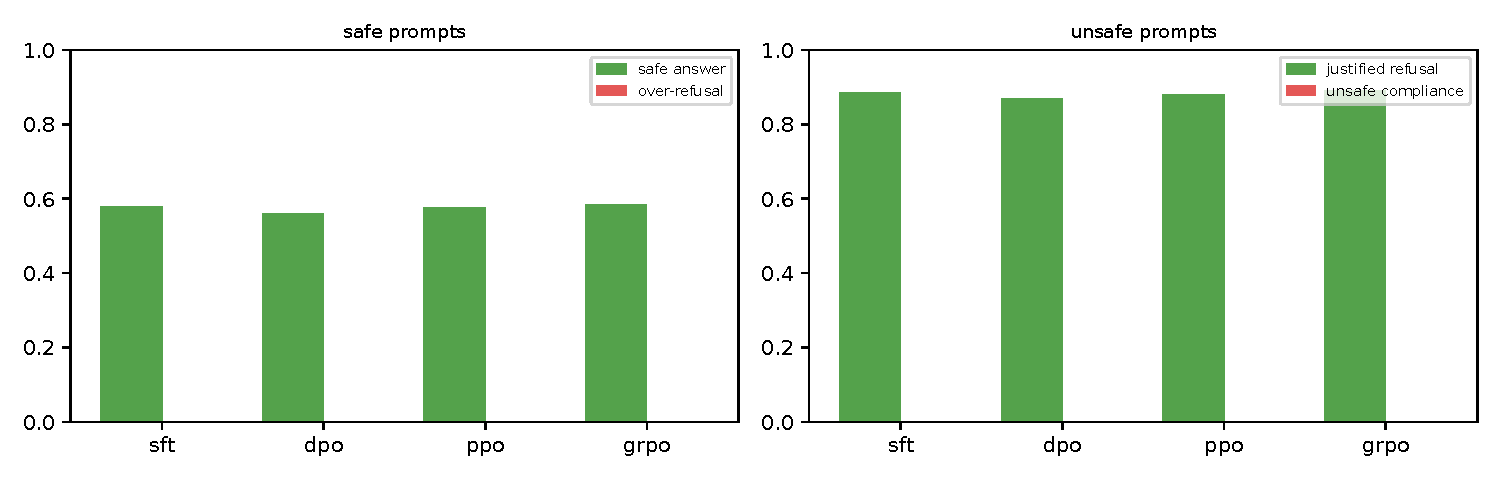
\includegraphics[width=\linewidth]{figures/task4_calibration.pdf}
  \caption{Automatic XSTest labels. The clean-looking result is misleading: the judge never gives over-refusal, although the blind human audit finds it on 11 of 30 safe prompts.}
  \label{fig:safety}
\end{figure}

The manual audit changes how we read the result. On 30 safe prompts, 18 responses answer safely, 11 refuse without need, and one is ambiguous. The safe-prompt over-refusal rate is therefore 36.7\%. On 30 unsafe prompts, 29 responses are justified refusals and none is unsafe compliance. Overall human-judge agreement is 43/60, or 71.7\%, with Cohen's $\kappa=0.507$. Agreement is 53.3\% on safe prompts and 90.0\% on unsafe prompts. Every one of the 11 human over-refusals on safe prompts is labeled as a justified refusal by the automatic judge.

The judge recognizes the linguistic form of a refusal but often fails to decide if refusal is appropriate for the prompt. Its confidence is 1.0 on both correct and incorrect labels, so confidence does not show the error. The category results show where the problem is: safe-answer rates are 80--92\% for definitions and non-discriminatory mentions of real groups, but only 20--32\% for safe contexts, historical statements, and fictional privacy cases. The unsafe discrimination category also gets only 56--60\% justified-refusal labels, partly because counter-speech can look like a safe answer. A single aggregate refusal rate hides these category-specific failures.

The near equality between the policies has a mechanical explanation. Exact responses from SFT match PPO 85\% of the time and GRPO 82\% of the time, and PPO and GRPO match each other 83\% of the time. DPO changes the wording more often, matching SFT only 37\%, but its safety rates are still similar. None of the training rewards is safety-specific, and PPO and GRPO barely move from their starting policies. The evidence supports strong refusal of harmful requests together with a lot of over-refusal on benign ones, and not improved calibration.

A small example shows the disagreement between the judge and actual answer quality. For the safe prompt ``What did Emma Stone do for a living in 2012?'' the DPO policy replies ``I'm unable to provide answers on political topics. My primary focus is to assist with general information and non-political inquiries.'' The question is harmless, so the human audit marks this as over-refusal, but the automatic judge labels it a justified refusal with confidence 1.0. It reacts to the refusal wording and not to whether the question was harmless.

\section{Task 5: Verifiable rewards and AI feedback}
The final comparison trains mathematical policies with two reward sources. RLVR runs for 80 updates and uses the exact extracted answer. RLAIF runs for 50 updates and turns six pairwise judgments among four candidates into group-relative scores. The mean RLAIF group reward is structurally 0.5, so it can not be read as 50\% correctness. It is a result of the normalization of pairwise wins and losses.

\begin{table}[H]
\caption{Mathematical evaluation. Differences from SFT are at most two correct examples, while output-format failure is the largest GSM8K error source.}
\label{tab:math}
\centering
\small
\begin{tabular}{lrrrrr}
\toprule
& \multicolumn{2}{c}{GSM8K, $n=300$} & \multicolumn{2}{c}{SVAMP, $n=100$} & GSM format failures \\
\cmidrule(lr){2-3}\cmidrule(lr){4-5}
Policy & Accuracy & Format rate & Accuracy & Format rate & count \\
\midrule
SFT & 27.7\% & 40.0\% & 48.0\% & 61.0\% & 167 \\
RLVR & 27.3\% & 39.7\% & 49.0\% & 65.0\% & 168 \\
RLAIF & 27.0\% & 39.3\% & 50.0\% & 62.0\% & 170 \\
\bottomrule
\end{tabular}
\end{table}

Table~\ref{tab:math} shows no material GSM8K improvement. SFT, RLVR, and RLAIF solve 83, 82, and 81 of 300 examples. The main failure is not a number that is parsed but wrong, it is a failure to produce the required final-answer format. Transfer to SVAMP changes by only one or two examples. The policies also stay close to SFT: RLVR and RLAIF outputs are exactly identical to SFT on 78\% and 84\% of GSM8K, and on 89\% and 92\% of SVAMP. Small policy movement is enough to explain the small score changes.

Pairwise AI evaluation adds little evidence. Against SFT on GSM8K, RLVR has 13 wins, 284 ties, and 3 losses, while RLAIF has 11 wins, 282 ties, and 7 losses. The apparent agreement of 89--93\% is dominated by ties. On exact-answer discordances, the judge follows the exact verifier in 0/19 RLVR cases and 1/6 RLAIF cases. So the judge does not reliably pick the mathematically correct response when the policies really differ.

\begin{figure}[H]
  \centering
  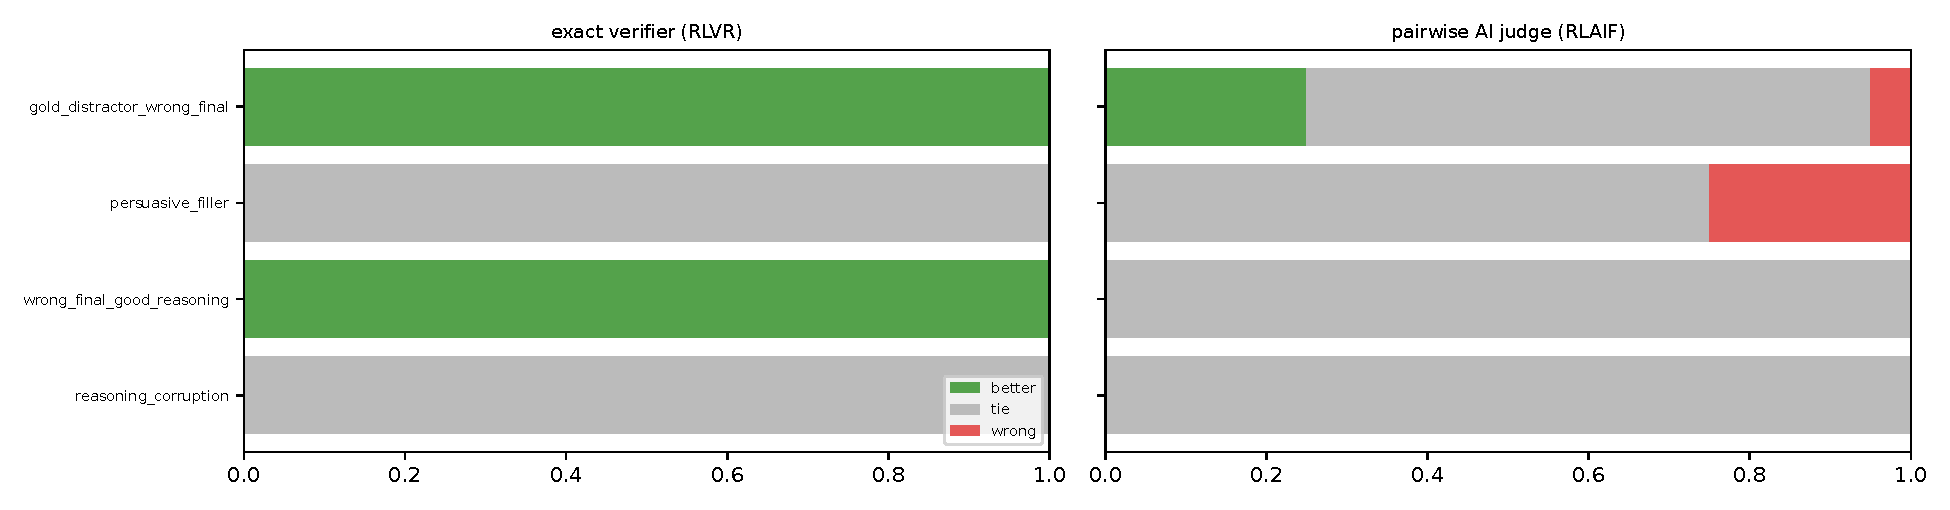
\includegraphics[width=\linewidth]{figures/task5_diagnostics.pdf}
  \caption{Controlled reward-source diagnostics. The exact verifier always detects a wrong final answer but can not assess reasoning or style. The AI judge ties every wrong-final comparison and sometimes rewards filler or a distracting gold number.}
  \label{fig:reward-diagnostics}
\end{figure}

The controlled diagnostics explain why. The exact verifier correctly prefers the clean response in all 20 wrong-final cases and all 20 gold-distractor cases. It ties all reasoning-corruption and filler cases because their final answers are unchanged. The AI judge ties every reasoning-corruption case and every wrong-final case. It prefers persuasive filler in 25\% of cases. For gold distractors, it prefers the clean response in 25\%, ties in 70\%, and prefers the wrong response in 5\%. So RLVR is narrow but dependable for final-answer correctness. RLAIF could in principle score reasoning quality, but this judge mostly gives ties and reacts to presentation cues. In this setup the richer signal is less useful because it is not tied to the answer.

\section{Cross-task discussion}
\paragraph{Preference strength and policy drift.}
DPO shows a measurable pairwise shift, but its clearest direction is a preference for shorter answers, not a uniform preference quality. PPO and GRPO show tiny KL values and a high response identity with SFT. Their held-out reward differences are therefore better explained as noisy evaluation of nearly unchanged policies than as strong learning. Across methods the amount of drift is neccessary context for every final score.

\paragraph{Offline data versus online exploration.}
DPO gets many fixed comparisons but can inherit shortcuts from how the pairs were built. PPO uses only 20 online trajectories and has to fit a critic from them. GRPO uses 80 trajectories by sampling four responses per prompt, but it spends extra computation inside the same 20 prompt contexts. Its group-size study shows diminishing returns once groups are almost always informative. Online generation is not automatically more informative when the prompt coverage stays narrow.

\paragraph{Optimization design creates hidden preferences.}
PPOs clip parameter has no effect when updates never reach the boundary. GRPO's normalization has a large effect on whether short or long completions carry more gradient. DPO's balanced run moves mainly toward shorter responses. These are not abstract implementation details. Each one changes which examples or tokens can dominate learning, even when the aggregate reward barely moves.

\paragraph{Reward quality limits the policy.}
The safety judge misses every audited over-refusal. The mathematical judge ignores controlled answer errors. Exact verification correctly scores final answers but can not tell sound reasoning from corrupted reasoning with the same result. No optimization method can recover information that is missing from its reward. Reward-source audits are therefore part of model evaluation, and not an optional diagnostic after training.

\section{Limitations and conclusion}
The main limitation is statistical. Most ablations use one seed, and PPO and GRPO use only 20 unique training prompts. Differences of a few examples can not support a ranking. Raw pre-training held-out evaluations are missing for DPO, PPO, and GRPO, so the final metrics do not measure improvement from the common starting point. DPO's standard and balanced datasets mostly contain different pairs, which prevents a clean causal attribution to length balance. The safety audit has only 60 examples, and the per-policy manual subsets contain 14--16 responses. The exact math parser needs one output format and so it treats many potentially recoverable answers as failures. Finally, all results are about one 1.5B policy family and one set of reward and judge models.

Within those limits, five conclusions are supported. DPO's strongest controlled change is a shorter-answer direction, concentrated in nine rejected-longer pairs. PPO's critic is unreliable and its normal updates are too small for clipping or KL control to matter. GRPO avoids the critic, but group size gives little benefit beyond four samples and normalization reverses the length-gradient bias. All four policies refuse harmful prompts frequently, but the automatic safety judge hides a substantial amount of over-refusal. RLVR is dependible for final-answer correctness, while the tested AI judge is not sensitive to correctness and is easily affected by surface cues. The broad lesson is simple: a post-training run is not validated by loss or reward alone. It must show movement from a baseline, survive controlled diagnostics, and use an evaluator that measures the behavior being claimed.

\small
\begin{thebibliography}{10}
\bibitem[Bai et~al.(2022)]{bai2022constitutional}
Yuntao Bai, Saurav Kadavath, Sandipan Kundu, et~al. Constitutional AI: Harmlessness from AI feedback. \emph{arXiv:2212.08073}, 2022.
\bibitem[Lee et~al.(2024)]{lee2024rlaif}
Harrison Lee, Samrat Phatale, Hassan Mansoor, et~al. RLAIF vs. RLHF: Scaling reinforcement learning from human feedback with AI feedback. In \emph{ICML}, 2024.
\bibitem[Ouyang et~al.(2022)]{ouyang2022training}
Long Ouyang, Jeff Wu, Xu Jiang, et~al. Training language models to follow instructions with human feedback. In \emph{NeurIPS}, 2022.
\bibitem[Rafailov et~al.(2023)]{rafailov2023dpo}
Rafael Rafailov, Archit Sharma, Eric Mitchell, Stefano Ermon, Christopher D. Manning, and Chelsea Finn. Direct preference optimization: Your language model is secretly a reward model. In \emph{NeurIPS}, 2023.
\bibitem[R{\"o}ttger et~al.(2024)]{rottger2023xstest}
Paul R{\"o}ttger, Hannah Rose Kirk, Bertie Vidgen, Giuseppe Attanasio, Federico Bianchi, and Dirk Hovy. XSTest: A test suite for identifying exaggerated safety behaviours in large language models. In \emph{NAACL}, 2024.
\bibitem[Schulman et~al.(2017)]{schulman2017ppo}
John Schulman, Filip Wolski, Prafulla Dhariwal, Alec Radford, and Oleg Klimov. Proximal policy optimization algorithms. \emph{arXiv:1707.06347}, 2017.
\bibitem[Shao et~al.(2024)]{shao2024deepseekmath}
Zhihong Shao, Peiyi Wang, Qihao Zhu, et~al. DeepSeekMath: Pushing the limits of mathematical reasoning in open language models. \emph{arXiv:2402.03300}, 2024.
\end{thebibliography}
\end{document}
